\documentclass{gwiki}

\Title{TikZ string diagrams demo}
\Tags{tikz, visualization, category theory}
\Aliases{TikZ demo, string diagram examples}
\Topics{String diagrams, coupons, patterns, arrows, color schemes, quick reference examples.}

\begin{document}

\NoteHeader

\begin{idea}
The \texttt{tz.sty} package provides convenient macros for drawing string diagrams, commutative diagrams, and other mathematical visualizations using TikZ, with support for layers, patterns, and specialized node styles.
\end{idea}

\section{Basic String Diagrams}

The \texttt{tz.sty} package provides inline TikZ via the \verb|\tz{}| command and the \texttt{tkz} environment. Here's a simple example:

\begin{center}
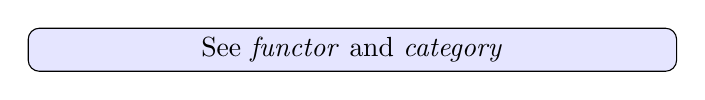
\begin{tikzpicture}
  \node[draw, rounded corners, fill=blue!10, text width=8cm, align=center] at (0,0) {See \textit{functor} and \textit{category}};
\end{tikzpicture}
\end{center}

\begin{example}[Inline diagram]
A morphism can be drawn inline:
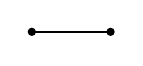
\begin{tikzpicture}[baseline=-0.5ex]
  \draw[thick] (0,0) -- (1,0); 
  \fill (0,0) circle (1.5pt); 
  \fill (1,0) circle (1.5pt);
\end{tikzpicture}
\end{example}

\section{Coupons and String Diagrams}

String diagrams use coupons (boxes) connected by strands:

\begin{center}
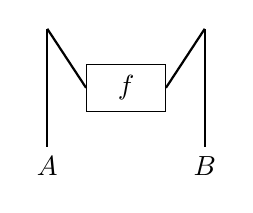
\begin{tikzpicture}
  % Draw strands
  \draw[thick] (0,0) -- (0,1.5);
  \draw[thick] (2,0) -- (2,1.5);

  % Draw coupon
  \node[draw, fill=white, minimum width=1cm, minimum height=0.6cm] (f) at (1,0.75) {$f$};

  % Connect to coupon
  \draw[thick] (0,1.5) -- (f.west);
  \draw[thick] (2,1.5) -- (f.east);

  % Label endpoints
  \node[below] at (0,0) {$A$};
  \node[below] at (2,0) {$B$};
\end{tikzpicture}
\end{center}

\section{Patterns and Regions}

The package includes several pattern styles for indicating different types of regions:

\begin{center}
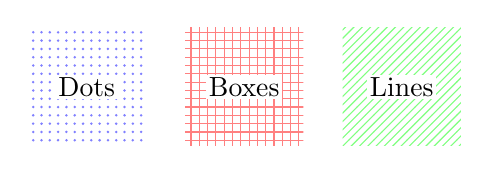
\begin{tikzpicture}
  \usetikzlibrary{patterns}
  \fill[pattern=dots, pattern color=blue!50] (0,0) rectangle (1.5,1.5);
  \fill[pattern=grid, pattern color=red!50] (2,0) rectangle (3.5,1.5);
  \fill[pattern=north east lines, pattern color=green!50] (4,0) rectangle (5.5,1.5);

  \node[fill=white, inner sep=1pt] at (0.75,0.75) {Dots};
  \node[fill=white, inner sep=1pt] at (2.75,0.75) {Boxes};
  \node[fill=white, inner sep=1pt] at (4.75,0.75) {Lines};
\end{tikzpicture}
\end{center}

\section{Arrow Styles}

Various arrow decorations are available:

\begin{center}
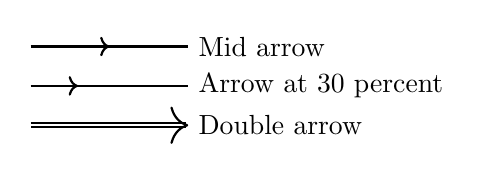
\begin{tikzpicture}
  \usetikzlibrary{decorations.markings, arrows.meta}
  \begin{scope}[decoration={markings, mark=at position 0.5 with {\arrow{>}}}] 
      \draw[thick, postaction={decorate}] (0,0) -- (2,0) node[right] {Mid arrow};
  \end{scope}

  \begin{scope}[decoration={markings, mark=at position 0.3 with {\arrow{>}}}]
      \draw[thick, postaction={decorate}] (0,-.5) -- (2,-.5) node[right] {Arrow at 30 percent};
  \end{scope}
  
  \draw[thick, double, ->] (0,-1) -- (2,-1) node[right] {Double arrow};
\end{tikzpicture}
\end{center}

\section{Knot Diagrams}

Drawing overcrossings and undercrossings:

\begin{center}
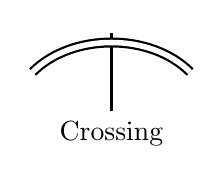
\begin{tikzpicture}
  % Second strand (goes under) - draw first for layering
  \draw[thick] (1,-0.5) -- (1,0.5);

  % White background for "over" effect
  \draw[double=white, double distance=2pt, thick] (0,0) .. controls (0.5,0.5) and (1.5,0.5) .. (2,0);
  
  \node[below] at (1,-0.5) {Crossing};
\end{tikzpicture}
\end{center}

\section{Color Schemes}

Predefined color scheme for consistency:

\begin{center}
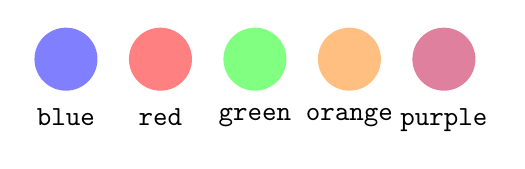
\begin{tikzpicture}
  \foreach \i/\col in {0/blue,1/red,2/green,3/orange,4/purple} {
    \fill[\col!50] (\i*1.2,0) circle (0.4);
    \node[below] at (\i*1.2,-0.5) {\texttt{\col}};
  }
\end{tikzpicture}
\end{center}

\section{Adjunctions (Snake Equations)}

String diagrams are particularly useful for expressing adjointness properties, such as the zigzag identities:

\begin{center}
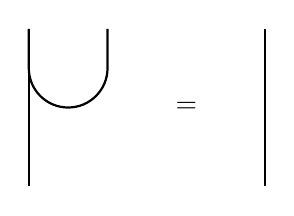
\begin{tikzpicture}
  % Left hand side
  \draw[thick] (0,2) -- (0,1.5) arc (180:360:0.5) -- (1,2);
  \draw[thick] (0,1.5) -- (0,0);
  
  % Right hand side
  \node at (2,1) {$=$};
  \draw[thick] (3,2) -- (3,0);
\end{tikzpicture}
\end{center}

\section{Commutative Diagrams}

We can use \texttt{tikz-cd} for commutative diagrams:

\begin{center}
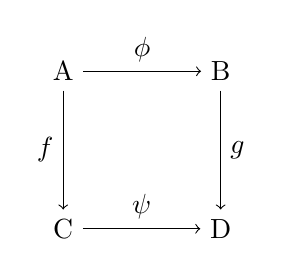
\begin{tikzpicture}
  \node (A) at (0,2) {A};
  \node (B) at (2,2) {B};
  \node (C) at (0,0) {C};
  \node (D) at (2,0) {D};
  
  \draw[->] (A) -- node[above] {$\phi$} (B);
  \draw[->] (A) -- node[left] {$f$} (C);
  \draw[->] (B) -- node[right] {$g$} (D);
  \draw[->] (C) -- node[above] {$\psi$} (D);
\end{tikzpicture}
\end{center}

\section{Function Plots}

TikZ can also plot functions:

\begin{center}
\begin{tikzpicture}
  \draw[->] (-0.2,0) -- (3,0) node[right] {$x$};
  \draw[->] (0,-0.2) -- (0,2) node[above] {$f(x)$};
  \draw[domain=0:2.5,smooth,variable=\x,blue,thick] plot ({\x},{0.25*\x*\x});
  \node[blue, right] at (2.5, 1.56) {$y = \frac{x^2}{4}$};
\end{tikzpicture}
\end{center}

\section{Conclusion}

The \texttt{tz.sty} package integrates seamlessly with GWiki's document class, providing powerful tools for mathematical visualization while maintaining clean, readable source code.

\SeeAlso{category,functor}

\References

\Footer

\end{document}
